\documentclass[twoside]{book}

% Packages required by doxygen
\usepackage{fixltx2e}
\usepackage{calc}
\usepackage{doxygen}
\usepackage[export]{adjustbox} % also loads graphicx
\usepackage{graphicx}
\usepackage[utf8]{inputenc}
\usepackage{makeidx}
\usepackage{multicol}
\usepackage{multirow}
\PassOptionsToPackage{warn}{textcomp}
\usepackage{textcomp}
\usepackage[nointegrals]{wasysym}
\usepackage[table]{xcolor}

% Font selection
\usepackage[T1]{fontenc}
\usepackage[scaled=.90]{helvet}
\usepackage{courier}
\usepackage{amssymb}
\usepackage{sectsty}
\renewcommand{\familydefault}{\sfdefault}
\allsectionsfont{%
  \fontseries{bc}\selectfont%
  \color{darkgray}%
}
\renewcommand{\DoxyLabelFont}{%
  \fontseries{bc}\selectfont%
  \color{darkgray}%
}
\newcommand{\+}{\discretionary{\mbox{\scriptsize$\hookleftarrow$}}{}{}}

% Page & text layout
\usepackage{geometry}
\geometry{%
  a4paper,%
  top=2.5cm,%
  bottom=2.5cm,%
  left=2.5cm,%
  right=2.5cm%
}
\tolerance=750
\hfuzz=15pt
\hbadness=750
\setlength{\emergencystretch}{15pt}
\setlength{\parindent}{0cm}
\setlength{\parskip}{3ex plus 2ex minus 2ex}
\makeatletter
\renewcommand{\paragraph}{%
  \@startsection{paragraph}{4}{0ex}{-1.0ex}{1.0ex}{%
    \normalfont\normalsize\bfseries\SS@parafont%
  }%
}
\renewcommand{\subparagraph}{%
  \@startsection{subparagraph}{5}{0ex}{-1.0ex}{1.0ex}{%
    \normalfont\normalsize\bfseries\SS@subparafont%
  }%
}
\makeatother

% Headers & footers
\usepackage{fancyhdr}
\pagestyle{fancyplain}
\fancyhead[LE]{\fancyplain{}{\bfseries\thepage}}
\fancyhead[CE]{\fancyplain{}{}}
\fancyhead[RE]{\fancyplain{}{\bfseries\leftmark}}
\fancyhead[LO]{\fancyplain{}{\bfseries\rightmark}}
\fancyhead[CO]{\fancyplain{}{}}
\fancyhead[RO]{\fancyplain{}{\bfseries\thepage}}
\fancyfoot[LE]{\fancyplain{}{}}
\fancyfoot[CE]{\fancyplain{}{}}
\fancyfoot[RE]{\fancyplain{}{\bfseries\scriptsize Generated by Doxygen }}
\fancyfoot[LO]{\fancyplain{}{\bfseries\scriptsize Generated by Doxygen }}
\fancyfoot[CO]{\fancyplain{}{}}
\fancyfoot[RO]{\fancyplain{}{}}
\renewcommand{\footrulewidth}{0.4pt}
\renewcommand{\chaptermark}[1]{%
  \markboth{#1}{}%
}
\renewcommand{\sectionmark}[1]{%
  \markright{\thesection\ #1}%
}

% Indices & bibliography
\usepackage{natbib}
\usepackage[titles]{tocloft}
\setcounter{tocdepth}{3}
\setcounter{secnumdepth}{5}
\makeindex

% Hyperlinks (required, but should be loaded last)
\usepackage{ifpdf}
\ifpdf
  \usepackage[pdftex,pagebackref=true]{hyperref}
\else
  \usepackage[ps2pdf,pagebackref=true]{hyperref}
\fi
\hypersetup{%
  colorlinks=true,%
  linkcolor=blue,%
  citecolor=blue,%
  unicode%
}

% Custom commands
\newcommand{\clearemptydoublepage}{%
  \newpage{\pagestyle{empty}\cleardoublepage}%
}

\usepackage{caption}
\captionsetup{labelsep=space,justification=centering,font={bf},singlelinecheck=off,skip=4pt,position=top}

%===== C O N T E N T S =====

\begin{document}

% Titlepage & ToC
\hypersetup{pageanchor=false,
             bookmarksnumbered=true,
             pdfencoding=unicode
            }
\pagenumbering{roman}
\begin{titlepage}
\vspace*{7cm}
\begin{center}%
{\Large Fun\+Robo\+Tugboat }\\
\vspace*{1cm}
{\large Generated by Doxygen 1.8.11}\\
\end{center}
\end{titlepage}
\clearemptydoublepage
\tableofcontents
\clearemptydoublepage
\pagenumbering{arabic}
\hypersetup{pageanchor=true}

%--- Begin generated contents ---
\chapter{Pixy2 Setup Instructions}
\label{md_Pixy2Info}
\hypertarget{md_Pixy2Info}{}
Following\+: \href{https://pixycam.com/downloads-pixy2/}{\tt https\+://pixycam.\+com/downloads-\/pixy2/}

\subsubsection*{Notes\+:}

If after {\ttfamily cd ../../../build/pixymon/bin/} you get the error {\ttfamily bash\+: cd\+: ../../../build/pixymon/bin/\+: No such file or directory} try using {\ttfamily cd $\sim$/pixy2/build/pixymon} instead.

Arduino Setup\+: \href{https://docs.pixycam.com/wiki/doku.php?id=wiki:v2:hooking_up_pixy_to_a_microcontroller_-28like_an_arduino-29}{\tt https\+://docs.\+pixycam.\+com/wiki/doku.\+php?id=wiki\+:v2\+:hooking\+\_\+up\+\_\+pixy\+\_\+to\+\_\+a\+\_\+microcontroller\+\_\+-\/28like\+\_\+an\+\_\+arduino-\/29}

After you extract the files, you will have a Pixy2 folder in your downloads. Move this folder to the Arduino/libraries folder.

\section*{Pixy2 Library usage}


\begin{DoxyItemize}
\item Include\+: {\ttfamily \#include $<$Pixy2.\+h$>$}
\item Object Declaration\+: {\ttfamily Pixy2 pixy;}
\item Updating pixy\+: {\ttfamily pixy.\+ccc.\+get\+Blocks();}
\item Number of detected objects\+: {\ttfamily pixy.\+ccc.\+num\+Blocks}
\item Printing info\+: {\ttfamily pixy.\+ccc.\+blocks\mbox{[}i\mbox{]}.print()}
\item Accessing data\+: {\ttfamily pixy.\+ccc.\+blocks\mbox{[}i\mbox{]}.$<$attribute$>$} (ex\+: {\ttfamily pixy.\+ccc.\+blocks\mbox{[}i\mbox{]}.m\+\_\+x})
\begin{DoxyItemize}
\item Attributes Include\+:
\begin{DoxyItemize}
\item {\ttfamily uint16\+\_\+t m\+\_\+signature} -\/ signature number -\/ If we have red registered as 1 and blue registered as 2, then these will be printed accordingly
\item {\ttfamily uint16\+\_\+t m\+\_\+x}
\item {\ttfamily uint16\+\_\+t m\+\_\+y}
\item {\ttfamily uint16\+\_\+t m\+\_\+width}
\item {\ttfamily uint16\+\_\+t m\+\_\+height}
\item {\ttfamily int16\+\_\+t m\+\_\+angle}
\item {\ttfamily uint8\+\_\+t m\+\_\+index}
\item {\ttfamily uint8\+\_\+t m\+\_\+age} 
\end{DoxyItemize}
\end{DoxyItemize}
\end{DoxyItemize}
\chapter{Fun\+Robo\+Tugboat}
\label{md_README}
\hypertarget{md_README}{}
Autonomous \hyperlink{class_tugboat}{Tugboat} -\/ Final project for Fundamentals of Robotics class, Fall 2018

\subsection*{Sensor Objects}

\subsubsection*{\hyperlink{class_i_r}{IR}}

\subparagraph*{Methods\+:}


\begin{DoxyItemize}
\item {\ttfamily void init()} -\/ initializes an \hyperlink{class_i_r}{IR} sensor, sets pin mode
\item {\ttfamily void update()} -\/ updates \hyperlink{class_i_r}{IR} data and saves it into data attribute
\item {\ttfamily void print()} -\/ prints the data
\end{DoxyItemize}

\subparagraph*{Attributes\+:}


\begin{DoxyItemize}
\item {\ttfamily int pin} -\/ analog in pin \hyperlink{class_i_r}{IR} is plugged into
\item {\ttfamily int x\+\_\+offset} -\/ not yet implemented
\item {\ttfamily int y\+\_\+offset} -\/ not yet implemented
\item {\ttfamily int heading} -\/ not yet implemented
\item {\ttfamily int data} -\/ \hyperlink{class_i_r}{IR} reading in cm
\end{DoxyItemize}

\subsubsection*{\hyperlink{class_pixycam}{Pixycam}}


\begin{DoxyItemize}
\item not yet implemented
\end{DoxyItemize}

\subsubsection*{\hyperlink{class_sonar}{Sonar}}

\subparagraph*{Methods\+:}


\begin{DoxyItemize}
\item {\ttfamily void init()} -\/ initializes an sonar sensor, sets pin mode
\item {\ttfamily void update()} -\/ updates sonar data and saves it into data attribute
\item {\ttfamily void print()} -\/ prints the data
\end{DoxyItemize}

\subparagraph*{Attributes\+:}


\begin{DoxyItemize}
\item {\ttfamily int pin} -\/ P\+WM pin sonar is plugged into
\item {\ttfamily int x\+\_\+offset} -\/ not yet implemented
\item {\ttfamily int y\+\_\+offset} -\/ not yet implemented
\item {\ttfamily int heading} -\/ not yet implemented
\item {\ttfamily int data} -\/ \hyperlink{class_i_r}{IR} reading in cm
\end{DoxyItemize}

\subsection*{Platform-\/dependent Objects}

\subsubsection*{\hyperlink{class_sensors}{Sensors}}

This object contains all the sensors and pin values for our specific tugboat configuration. This was made to streamline the sensor data flows from the sensors to the tugboat, especially when sensors get put on different arduinos. All pin values for sensors are stored in {\ttfamily \hyperlink{_sensors_8h_source}{Sensors.\+h}}

\subparagraph*{Methods\+:}


\begin{DoxyItemize}
\item {\ttfamily void init()} -\/ initializes all sensors, sets all pin modes
\item {\ttfamily void update()} -\/ updates sonar data and saves it into data attribute
\item {\ttfamily void print()} -\/ prints the data
\end{DoxyItemize}

\subparagraph*{Attributes\+:}


\begin{DoxyItemize}
\item {\ttfamily \hyperlink{class_i_r}{IR} ir\+\_\+0} -\/ \hyperlink{class_i_r}{IR} object 0
\item ...
\item {\ttfamily \hyperlink{class_i_r}{IR} ir\+\_\+5} -\/ \hyperlink{class_i_r}{IR} object 5
\item {\ttfamily \hyperlink{class_sonar}{Sonar} sonar\+\_\+0} -\/ \hyperlink{class_sonar}{Sonar} object 0
\item ...
\item {\ttfamily \hyperlink{class_sonar}{Sonar} sonar\+\_\+2} -\/ \hyperlink{class_sonar}{Sonar} object 2
\item {\ttfamily \hyperlink{class_pixycam}{Pixycam} pixycam} -\/ \hyperlink{class_pixycam}{Pixycam} object
\end{DoxyItemize}

\subsubsection*{\hyperlink{class_tugboat}{Tugboat}}

\subparagraph*{Methods\+:}


\begin{DoxyItemize}
\item {\ttfamily void init()} -\/ initializes a boat, also calls init function for sensors
\item {\ttfamily void update()} -\/ calls update function for all sensors
\item {\ttfamily void move()} -\/ moves the boat based on heading
\item {\ttfamily void print()} -\/ not yet implemented
\item {\ttfamily void state\+Controller()} -\/ sets the state for the boat and calls appropriate function
\item {\ttfamily void stop()}
\item {\ttfamily void idle()}
\item {\ttfamily void avoid()}
\item {\ttfamily void lwall()}
\item {\ttfamily void rwall()}
\item {\ttfamily void lcircle()}
\item {\ttfamily void rcircle()}
\item {\ttfamily void chase()}
\item {\ttfamily void search()}
\item {\ttfamily void set\+Prop\+Speed(int speed\+Percentage)}
\item {\ttfamily void set\+Heading(int deg\+Heading)}
\end{DoxyItemize}

\subparagraph*{Attributes\+:}


\begin{DoxyItemize}
\item {\ttfamily \hyperlink{class_sensors}{Sensors} sensors}
\item {\ttfamily int heading} -\/ Heading value in degrees
\item {\ttfamily int velocity} -\/ Velocity value between -\/100 and 100
\item {\ttfamily int state = 0} -\/ Integer representing state
\begin{DoxyItemize}
\item State 1\+: stop
\item State 2\+: idle
\item State 3\+: avoid -\/ use all sensor data to move to a safer position
\item State 4\+: lwall -\/ follow wall on left of boat
\item State 5\+: rwall -\/ follow wall on right of boat
\item State 6\+: lcircle -\/ circumnavigate an object on left of boat
\item State 7\+: rcircle -\/ circumnavigate an object on right of boat
\item State 8\+: chase
\item State 9\+: search
\item State Other\+: stop
\end{DoxyItemize}
\end{DoxyItemize}

\subsection*{Now With Arduino Comms\+:}

We\textquotesingle{}re using the Easy\+Transfer library for inter-\/\+Arduino communications. A link to getting this library set up is here -\/$>$ \href{https://github.com/EverardoG/Arduino-EasyTransfer}{\tt https\+://github.\+com/\+Everardo\+G/\+Arduino-\/\+Easy\+Transfer}.

Arduino 1 passes the {\ttfamily pixydata} object to Arduino 2. Arduino 2 packs the data from {\ttfamily pixydata} and the information collected by its low level sensor suite into {\ttfamily sensedata}. Arduino 2 sends \textquotesingle{}sensedata\textquotesingle{} to Arduino 3. This is all done using the Tx and Rx pins on the Arduinos. This means it uses the same serial channel that you use for the Arduino Serial Monitor. The T\+H\+I\+N\+K/ A\+CT Arduino can print to Serial, but sending it anything through the Serial monitor will confuse it.

\subsubsection*{Attributes of pixydata}


\begin{DoxyItemize}
\item {\ttfamily unsigned long timestamp1} -\/ millisecond timestamp from Arduino 1 when it sent {\ttfamily pixydata} (This was just to test functionality)
\end{DoxyItemize}

We will add more to this once we figure out exactly what pieces of data we want from the pixycam.

\subsubsection*{Attributes of sensedata}


\begin{DoxyItemize}
\item {\ttfamily unsigned long timestamp1} -\/ millisecond timestamp from Arduino 1 when it sent {\ttfamily pixydata} (This was just to test functionality)
\item {\ttfamily unsigned long timestamp2} -\/ millisecond timestamp from Arduino 2 when it sent {\ttfamily sensedata} (This was just to test functionality)
\item {\ttfamily int ir\+\_\+0\+\_\+data} -\/ meters measured by \hyperlink{class_i_r}{IR} 0
\item {\ttfamily int ir\+\_\+1\+\_\+data} -\/ meters measured by \hyperlink{class_i_r}{IR} 1
\item {\ttfamily int ir\+\_\+2\+\_\+data} -\/ meters measured by \hyperlink{class_i_r}{IR} 2
\item {\ttfamily int ir\+\_\+3\+\_\+data} -\/ meters measured by \hyperlink{class_i_r}{IR} 3
\item {\ttfamily int ir\+\_\+4\+\_\+data} -\/ meters measured by \hyperlink{class_i_r}{IR} 4
\item {\ttfamily int ir\+\_\+5\+\_\+data} -\/ meters measured by \hyperlink{class_i_r}{IR} 5
\item {\ttfamily sonar\+\_\+0\+\_\+data} -\/ meters measured by sonar 0
\item {\ttfamily sonar\+\_\+1\+\_\+data} -\/ meters measured by sonar 1
\item {\ttfamily sonar\+\_\+2\+\_\+data} -\/ meters measured by sonar 2
\end{DoxyItemize}

There will be more here once we integrate actual values from the pixycam.

\subsection*{Now with X\+Bee Comms}

We can now communicate with our boat remotely! It\textquotesingle{}s awesome! We use an {\ttfamily Xbee} object on Arduino 3 to communicate via X\+Bee.

For it to work, you need to install the X\+Bee software on your laptop first. Here\textquotesingle{}s a really great walkthrough on that -\/$>$ \href{https://github.com/olinrobotics/main/wiki/XBee-Radios}{\tt https\+://github.\+com/olinrobotics/main/wiki/\+X\+Bee-\/\+Radios}. Once you have that set up, here\textquotesingle{}s the step-\/by-\/step guide to setting up comms.

\subsubsection*{Setup}

\paragraph*{Boat Side}


\begin{DoxyEnumerate}
\item Upload code to each Arduino. Arduino 1 is the pixy cam arduino. Arduino 2 is the low level sensing arduino. Arduino 3 is the T\+H\+I\+N\+K/\+A\+CT arduino.
\item Make sure that all arduinos are connected to eachother properly. Arduino 1 Tx -\/$>$ Arduino 2 Rx Arduino 2 Tx -\/$>$ Arduino 3 Rx
\item Verify that the X\+Bee is indeed plugged into Arduino 3.
\item Turn on the boat.
\end{DoxyEnumerate}

\paragraph*{Laptop Side}


\begin{DoxyEnumerate}
\item Connect the O\+CU X\+Bee to your laptop via the adaptor board.
\item Open up the X\+C\+T\+U.\+desktop software. Remember, you need to use {\ttfamily sudo X\+C\+TU ./\+X\+C\+TU.desktop} to make it work.
\item Click \char`\"{}\+Add a Radio Module\char`\"{} in the upper left hand corner. Add the O\+CU X\+Bee. It should show up with \char`\"{}\+O\+C\+U\char`\"{} as its name.
\item In the upper right, there\textquotesingle{}s a gear icon. Next to it is a computer/ terminal icon. Click it.
\item Now you\textquotesingle{}ll see three icons above the \char`\"{}\+Console Log\char`\"{}. Click \char`\"{}\+Open\char`\"{}. This makes it so that your laptop X\+Bee is now listening to the boat X\+Bee. You can also type into the \char`\"{}\+Console Log\char`\"{} to send commands to the boat!
\end{DoxyEnumerate}

\subsubsection*{Methods of X\+Bee Comms Object}


\begin{DoxyItemize}
\item {\ttfamily void begin(int baudrate)} -\/ sets the data baudrate for X\+Bee transmission
\item {\ttfamily void write(char array)} -\/ the boat will send out this char array to the X\+Bee channel
\item {\ttfamily int available()} -\/ returns the number of bytes avaiable to read from X\+Bee channel
\item {\ttfamily char read()} -\/ returns the character read on the X\+Bee channel (Someone should double check this, but for our purposes, this captures everything that matters)
\end{DoxyItemize}

\section*{To-\/do\+:}


\begin{DoxyItemize}
\item write behavior functions
\item put sensor object functions in separate folder when complete
\item determine if P\+WM signals alone would be good enough for sonars (will need other pins if sensors have conflict issues) and update code to reflect that
\item determine how \hyperlink{class_pixycam}{Pixycam} data is processed 
\end{DoxyItemize}
\chapter{Class Index}
\section{Class List}
Here are the classes, structs, unions and interfaces with brief descriptions\+:\begin{DoxyCompactList}
\item\contentsline{section}{\hyperlink{class_i_r}{IR} }{\pageref{class_i_r}}{}
\item\contentsline{section}{\hyperlink{class_pixycam}{Pixycam} }{\pageref{class_pixycam}}{}
\item\contentsline{section}{\hyperlink{struct_r_e_c_e_i_v_e___d_a_t_a___s_t_r_u_c_t_u_r_e}{R\+E\+C\+E\+I\+V\+E\+\_\+\+D\+A\+T\+A\+\_\+\+S\+T\+R\+U\+C\+T\+U\+RE} }{\pageref{struct_r_e_c_e_i_v_e___d_a_t_a___s_t_r_u_c_t_u_r_e}}{}
\item\contentsline{section}{\hyperlink{struct_r_e_c_i_e_v_e___d_a_t_a___s_t_r_u_c_t_u_r_e}{R\+E\+C\+I\+E\+V\+E\+\_\+\+D\+A\+T\+A\+\_\+\+S\+T\+R\+U\+C\+T\+U\+RE} }{\pageref{struct_r_e_c_i_e_v_e___d_a_t_a___s_t_r_u_c_t_u_r_e}}{}
\item\contentsline{section}{\hyperlink{struct_s_e_n_d___d_a_t_a___s_t_r_u_c_t_u_r_e}{S\+E\+N\+D\+\_\+\+D\+A\+T\+A\+\_\+\+S\+T\+R\+U\+C\+T\+U\+RE} }{\pageref{struct_s_e_n_d___d_a_t_a___s_t_r_u_c_t_u_r_e}}{}
\item\contentsline{section}{\hyperlink{class_sensors}{Sensors} }{\pageref{class_sensors}}{}
\item\contentsline{section}{\hyperlink{class_sonar}{Sonar} }{\pageref{class_sonar}}{}
\item\contentsline{section}{\hyperlink{class_tugboat}{Tugboat} }{\pageref{class_tugboat}}{}
\item\contentsline{section}{\hyperlink{class_wall_follow}{Wall\+Follow} }{\pageref{class_wall_follow}}{}
\end{DoxyCompactList}

\chapter{Class Documentation}
\hypertarget{class_i_r}{}\section{IR Class Reference}
\label{class_i_r}\index{IR@{IR}}
\subsection*{Public Member Functions}
\begin{DoxyCompactItemize}
\item 
void {\bfseries init} ()\hypertarget{class_i_r_a7c5d9ba17b7d3c26e4e284da1763d0a7}{}\label{class_i_r_a7c5d9ba17b7d3c26e4e284da1763d0a7}

\item 
void {\bfseries update} ()\hypertarget{class_i_r_acdde67e3ad75d030457be93fc2682999}{}\label{class_i_r_acdde67e3ad75d030457be93fc2682999}

\item 
void {\bfseries print} ()\hypertarget{class_i_r_a11b729611514f95ef01c115db86b27b3}{}\label{class_i_r_a11b729611514f95ef01c115db86b27b3}

\end{DoxyCompactItemize}
\subsection*{Public Attributes}
\begin{DoxyCompactItemize}
\item 
int {\bfseries pin} = 0\hypertarget{class_i_r_a638c3210a15cc10dc5a9753ba1bd21cf}{}\label{class_i_r_a638c3210a15cc10dc5a9753ba1bd21cf}

\item 
int {\bfseries x\+\_\+offset} = 0\hypertarget{class_i_r_a0d957c8d3488651c72085702b5beb5f2}{}\label{class_i_r_a0d957c8d3488651c72085702b5beb5f2}

\item 
int {\bfseries y\+\_\+offset} = 0\hypertarget{class_i_r_a80113b9db53ff9177fa0fdcd65cf7d62}{}\label{class_i_r_a80113b9db53ff9177fa0fdcd65cf7d62}

\item 
int {\bfseries heading} = 0\hypertarget{class_i_r_ad53c7f3e0582c9ddbbdfcf4a38e61f7e}{}\label{class_i_r_ad53c7f3e0582c9ddbbdfcf4a38e61f7e}

\item 
int {\bfseries data} = 0\hypertarget{class_i_r_aa144ad3dd59f51c81679379bb133deb4}{}\label{class_i_r_aa144ad3dd59f51c81679379bb133deb4}

\end{DoxyCompactItemize}


The documentation for this class was generated from the following files\+:\begin{DoxyCompactItemize}
\item 
Tugboat\+\_\+\+Arduino\+\_\+2/I\+R.\+h\item 
Tugboat\+\_\+\+Arduino\+\_\+2/I\+R.\+cpp\end{DoxyCompactItemize}

\hypertarget{class_pixycam}{}\section{Pixycam Class Reference}
\label{class_pixycam}\index{Pixycam@{Pixycam}}
\subsection*{Public Member Functions}
\begin{DoxyCompactItemize}
\item 
void {\bfseries init} ()\hypertarget{class_pixycam_a49da1e59eda420e02062cdd2faae457f}{}\label{class_pixycam_a49da1e59eda420e02062cdd2faae457f}

\item 
void {\bfseries update} ()\hypertarget{class_pixycam_adab9bbd0ec2d9a1171805ccac22ee858}{}\label{class_pixycam_adab9bbd0ec2d9a1171805ccac22ee858}

\item 
void {\bfseries print} ()\hypertarget{class_pixycam_a0de4d34b57257c283fe8350f16fa29b3}{}\label{class_pixycam_a0de4d34b57257c283fe8350f16fa29b3}

\end{DoxyCompactItemize}
\subsection*{Public Attributes}
\begin{DoxyCompactItemize}
\item 
Pixy {\bfseries pixy}\hypertarget{class_pixycam_aff7edc67f54c08390c786eb83186c962}{}\label{class_pixycam_aff7edc67f54c08390c786eb83186c962}

\item 
int {\bfseries x\+\_\+offset} = 0\hypertarget{class_pixycam_a079fccb432e32c49f85223069b9143b2}{}\label{class_pixycam_a079fccb432e32c49f85223069b9143b2}

\item 
int {\bfseries y\+\_\+offset} = 0\hypertarget{class_pixycam_a78db4ec4f2a2561c003868d37e1dc561}{}\label{class_pixycam_a78db4ec4f2a2561c003868d37e1dc561}

\item 
int {\bfseries heading} = 0\hypertarget{class_pixycam_aac007f3ff2cd4aa36c1c7fb036ac2449}{}\label{class_pixycam_aac007f3ff2cd4aa36c1c7fb036ac2449}

\item 
int {\bfseries data} = 0\hypertarget{class_pixycam_a0711c3ce000b0e99a19c4e827229c9f6}{}\label{class_pixycam_a0711c3ce000b0e99a19c4e827229c9f6}

\end{DoxyCompactItemize}


The documentation for this class was generated from the following files\+:\begin{DoxyCompactItemize}
\item 
Tugboat\+\_\+\+Arduino\+\_\+1/Pixycam.\+h\item 
Tugboat\+\_\+\+Arduino\+\_\+1/Pixycam.\+cpp\end{DoxyCompactItemize}

\hypertarget{struct_r_e_c_e_i_v_e___d_a_t_a___s_t_r_u_c_t_u_r_e}{}\section{R\+E\+C\+E\+I\+V\+E\+\_\+\+D\+A\+T\+A\+\_\+\+S\+T\+R\+U\+C\+T\+U\+RE Struct Reference}
\label{struct_r_e_c_e_i_v_e___d_a_t_a___s_t_r_u_c_t_u_r_e}\index{R\+E\+C\+E\+I\+V\+E\+\_\+\+D\+A\+T\+A\+\_\+\+S\+T\+R\+U\+C\+T\+U\+RE@{R\+E\+C\+E\+I\+V\+E\+\_\+\+D\+A\+T\+A\+\_\+\+S\+T\+R\+U\+C\+T\+U\+RE}}
\subsection*{Public Attributes}
\begin{DoxyCompactItemize}
\item 
unsigned long {\bfseries timestamp1}\hypertarget{struct_r_e_c_e_i_v_e___d_a_t_a___s_t_r_u_c_t_u_r_e_a321dd55121b07ecfc7902ba462f224cd}{}\label{struct_r_e_c_e_i_v_e___d_a_t_a___s_t_r_u_c_t_u_r_e_a321dd55121b07ecfc7902ba462f224cd}

\end{DoxyCompactItemize}


The documentation for this struct was generated from the following file\+:\begin{DoxyCompactItemize}
\item 
Tugboat\+\_\+\+Arduino\+\_\+2/Arduino\+Comms2.\+h\end{DoxyCompactItemize}

\hypertarget{struct_r_e_c_i_e_v_e___d_a_t_a___s_t_r_u_c_t_u_r_e}{}\section{R\+E\+C\+I\+E\+V\+E\+\_\+\+D\+A\+T\+A\+\_\+\+S\+T\+R\+U\+C\+T\+U\+RE Struct Reference}
\label{struct_r_e_c_i_e_v_e___d_a_t_a___s_t_r_u_c_t_u_r_e}\index{R\+E\+C\+I\+E\+V\+E\+\_\+\+D\+A\+T\+A\+\_\+\+S\+T\+R\+U\+C\+T\+U\+RE@{R\+E\+C\+I\+E\+V\+E\+\_\+\+D\+A\+T\+A\+\_\+\+S\+T\+R\+U\+C\+T\+U\+RE}}
\subsection*{Public Attributes}
\begin{DoxyCompactItemize}
\item 
unsigned long {\bfseries timestamp1}\hypertarget{struct_r_e_c_i_e_v_e___d_a_t_a___s_t_r_u_c_t_u_r_e_a55d09ebf5b034d4d197546a7a0294abb}{}\label{struct_r_e_c_i_e_v_e___d_a_t_a___s_t_r_u_c_t_u_r_e_a55d09ebf5b034d4d197546a7a0294abb}

\item 
unsigned long {\bfseries timestamp2}\hypertarget{struct_r_e_c_i_e_v_e___d_a_t_a___s_t_r_u_c_t_u_r_e_adfbab4bee916f32ebe38a934e0f0e875}{}\label{struct_r_e_c_i_e_v_e___d_a_t_a___s_t_r_u_c_t_u_r_e_adfbab4bee916f32ebe38a934e0f0e875}

\item 
int {\bfseries ir\+\_\+0\+\_\+data} = 0\hypertarget{struct_r_e_c_i_e_v_e___d_a_t_a___s_t_r_u_c_t_u_r_e_a48d33ddd33d317a3c884fd46ab5728ef}{}\label{struct_r_e_c_i_e_v_e___d_a_t_a___s_t_r_u_c_t_u_r_e_a48d33ddd33d317a3c884fd46ab5728ef}

\item 
int {\bfseries ir\+\_\+1\+\_\+data} = 0\hypertarget{struct_r_e_c_i_e_v_e___d_a_t_a___s_t_r_u_c_t_u_r_e_a36af77c0244987100ea09db2302b83be}{}\label{struct_r_e_c_i_e_v_e___d_a_t_a___s_t_r_u_c_t_u_r_e_a36af77c0244987100ea09db2302b83be}

\item 
int {\bfseries ir\+\_\+2\+\_\+data} = 0\hypertarget{struct_r_e_c_i_e_v_e___d_a_t_a___s_t_r_u_c_t_u_r_e_ab9c71c15e138e15b2f4351a41bccd2b9}{}\label{struct_r_e_c_i_e_v_e___d_a_t_a___s_t_r_u_c_t_u_r_e_ab9c71c15e138e15b2f4351a41bccd2b9}

\item 
int {\bfseries ir\+\_\+3\+\_\+data} = 0\hypertarget{struct_r_e_c_i_e_v_e___d_a_t_a___s_t_r_u_c_t_u_r_e_a6dd2d212efaf5be01d48d919f81bd524}{}\label{struct_r_e_c_i_e_v_e___d_a_t_a___s_t_r_u_c_t_u_r_e_a6dd2d212efaf5be01d48d919f81bd524}

\item 
int {\bfseries ir\+\_\+4\+\_\+data} = 0\hypertarget{struct_r_e_c_i_e_v_e___d_a_t_a___s_t_r_u_c_t_u_r_e_a633be90a6ae1f57798dcc9056ad92a4b}{}\label{struct_r_e_c_i_e_v_e___d_a_t_a___s_t_r_u_c_t_u_r_e_a633be90a6ae1f57798dcc9056ad92a4b}

\item 
int {\bfseries ir\+\_\+5\+\_\+data} = 0\hypertarget{struct_r_e_c_i_e_v_e___d_a_t_a___s_t_r_u_c_t_u_r_e_a62fee75f29560c03cc511848be988c9b}{}\label{struct_r_e_c_i_e_v_e___d_a_t_a___s_t_r_u_c_t_u_r_e_a62fee75f29560c03cc511848be988c9b}

\item 
int {\bfseries sonar\+\_\+0\+\_\+data} = 0\hypertarget{struct_r_e_c_i_e_v_e___d_a_t_a___s_t_r_u_c_t_u_r_e_a00e7a748f950d5aef837afbd3f4d2997}{}\label{struct_r_e_c_i_e_v_e___d_a_t_a___s_t_r_u_c_t_u_r_e_a00e7a748f950d5aef837afbd3f4d2997}

\item 
int {\bfseries sonar\+\_\+1\+\_\+data} = 0\hypertarget{struct_r_e_c_i_e_v_e___d_a_t_a___s_t_r_u_c_t_u_r_e_add6c622bdfc96b23e0e8016ee5292cbd}{}\label{struct_r_e_c_i_e_v_e___d_a_t_a___s_t_r_u_c_t_u_r_e_add6c622bdfc96b23e0e8016ee5292cbd}

\item 
int {\bfseries sonar\+\_\+2\+\_\+data} = 0\hypertarget{struct_r_e_c_i_e_v_e___d_a_t_a___s_t_r_u_c_t_u_r_e_a75f5f4198e628949f9cefc3922b921e1}{}\label{struct_r_e_c_i_e_v_e___d_a_t_a___s_t_r_u_c_t_u_r_e_a75f5f4198e628949f9cefc3922b921e1}

\end{DoxyCompactItemize}


The documentation for this struct was generated from the following file\+:\begin{DoxyCompactItemize}
\item 
Tugboat\+\_\+\+Arduino\+\_\+3/Arduino\+Comms3.\+h\end{DoxyCompactItemize}

\hypertarget{struct_s_e_n_d___d_a_t_a___s_t_r_u_c_t_u_r_e}{}\section{S\+E\+N\+D\+\_\+\+D\+A\+T\+A\+\_\+\+S\+T\+R\+U\+C\+T\+U\+RE Struct Reference}
\label{struct_s_e_n_d___d_a_t_a___s_t_r_u_c_t_u_r_e}\index{S\+E\+N\+D\+\_\+\+D\+A\+T\+A\+\_\+\+S\+T\+R\+U\+C\+T\+U\+RE@{S\+E\+N\+D\+\_\+\+D\+A\+T\+A\+\_\+\+S\+T\+R\+U\+C\+T\+U\+RE}}
\subsection*{Public Attributes}
\begin{DoxyCompactItemize}
\item 
unsigned long {\bfseries timestamp1}\hypertarget{struct_s_e_n_d___d_a_t_a___s_t_r_u_c_t_u_r_e_a0943fbe994d0eaaff6771d41e3894aae}{}\label{struct_s_e_n_d___d_a_t_a___s_t_r_u_c_t_u_r_e_a0943fbe994d0eaaff6771d41e3894aae}

\item 
unsigned long {\bfseries timestamp2}\hypertarget{struct_s_e_n_d___d_a_t_a___s_t_r_u_c_t_u_r_e_a52e8a50f9ae7333c68e9970119f419cc}{}\label{struct_s_e_n_d___d_a_t_a___s_t_r_u_c_t_u_r_e_a52e8a50f9ae7333c68e9970119f419cc}

\item 
int {\bfseries ir\+\_\+0\+\_\+data} = 0\hypertarget{struct_s_e_n_d___d_a_t_a___s_t_r_u_c_t_u_r_e_a67795fc35607eb2668e2671f0b06f1b2}{}\label{struct_s_e_n_d___d_a_t_a___s_t_r_u_c_t_u_r_e_a67795fc35607eb2668e2671f0b06f1b2}

\item 
int {\bfseries ir\+\_\+1\+\_\+data} = 0\hypertarget{struct_s_e_n_d___d_a_t_a___s_t_r_u_c_t_u_r_e_a257d908a7657c84eb118049186caf4e9}{}\label{struct_s_e_n_d___d_a_t_a___s_t_r_u_c_t_u_r_e_a257d908a7657c84eb118049186caf4e9}

\item 
int {\bfseries ir\+\_\+2\+\_\+data} = 0\hypertarget{struct_s_e_n_d___d_a_t_a___s_t_r_u_c_t_u_r_e_ad2baffc96bca820e409743ce9a6334de}{}\label{struct_s_e_n_d___d_a_t_a___s_t_r_u_c_t_u_r_e_ad2baffc96bca820e409743ce9a6334de}

\item 
int {\bfseries ir\+\_\+3\+\_\+data} = 0\hypertarget{struct_s_e_n_d___d_a_t_a___s_t_r_u_c_t_u_r_e_a2348f951c9e4d82af2ad0b70560f79cc}{}\label{struct_s_e_n_d___d_a_t_a___s_t_r_u_c_t_u_r_e_a2348f951c9e4d82af2ad0b70560f79cc}

\item 
int {\bfseries ir\+\_\+4\+\_\+data} = 0\hypertarget{struct_s_e_n_d___d_a_t_a___s_t_r_u_c_t_u_r_e_a6a86fa534d5b0cd1a9e604783d860867}{}\label{struct_s_e_n_d___d_a_t_a___s_t_r_u_c_t_u_r_e_a6a86fa534d5b0cd1a9e604783d860867}

\item 
int {\bfseries ir\+\_\+5\+\_\+data} = 0\hypertarget{struct_s_e_n_d___d_a_t_a___s_t_r_u_c_t_u_r_e_a1f03f46b1621ed4b2ed2f113108fe518}{}\label{struct_s_e_n_d___d_a_t_a___s_t_r_u_c_t_u_r_e_a1f03f46b1621ed4b2ed2f113108fe518}

\item 
int {\bfseries sonar\+\_\+0\+\_\+data} = 0\hypertarget{struct_s_e_n_d___d_a_t_a___s_t_r_u_c_t_u_r_e_a068e6175f21d5bbfdc5ea36c02e63383}{}\label{struct_s_e_n_d___d_a_t_a___s_t_r_u_c_t_u_r_e_a068e6175f21d5bbfdc5ea36c02e63383}

\item 
int {\bfseries sonar\+\_\+1\+\_\+data} = 0\hypertarget{struct_s_e_n_d___d_a_t_a___s_t_r_u_c_t_u_r_e_a5d8f2356332f1d8361ffa71439ad6409}{}\label{struct_s_e_n_d___d_a_t_a___s_t_r_u_c_t_u_r_e_a5d8f2356332f1d8361ffa71439ad6409}

\item 
int {\bfseries sonar\+\_\+2\+\_\+data} = 0\hypertarget{struct_s_e_n_d___d_a_t_a___s_t_r_u_c_t_u_r_e_a2712af20c5b2949c218afbe15f97745e}{}\label{struct_s_e_n_d___d_a_t_a___s_t_r_u_c_t_u_r_e_a2712af20c5b2949c218afbe15f97745e}

\end{DoxyCompactItemize}


The documentation for this struct was generated from the following files\+:\begin{DoxyCompactItemize}
\item 
Tugboat\+\_\+\+Arduino\+\_\+1/Arduino\+Comms1.\+h\item 
Tugboat\+\_\+\+Arduino\+\_\+2/Arduino\+Comms2.\+h\end{DoxyCompactItemize}

\hypertarget{class_sensors}{}\section{Sensors Class Reference}
\label{class_sensors}\index{Sensors@{Sensors}}


Collaboration diagram for Sensors\+:
\nopagebreak
\begin{figure}[H]
\begin{center}
\leavevmode
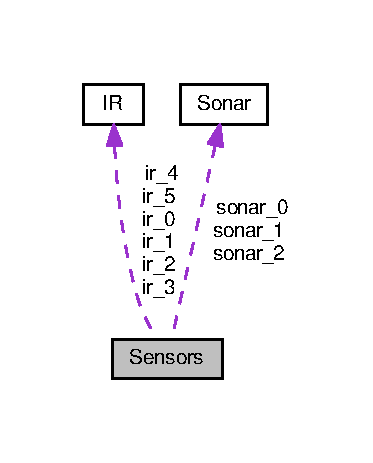
\includegraphics[width=179pt]{class_sensors__coll__graph}
\end{center}
\end{figure}
\subsection*{Public Member Functions}
\begin{DoxyCompactItemize}
\item 
void {\bfseries init} ()\hypertarget{class_sensors_a6dc9f66e4319c82649dc79cfa4e5ead8}{}\label{class_sensors_a6dc9f66e4319c82649dc79cfa4e5ead8}

\item 
void {\bfseries update} ()\hypertarget{class_sensors_af0290d09b1ae4dd7726a2a6613bf354b}{}\label{class_sensors_af0290d09b1ae4dd7726a2a6613bf354b}

\item 
void {\bfseries print} ()\hypertarget{class_sensors_ad38384b568dac4c2f656a78c28464e9a}{}\label{class_sensors_ad38384b568dac4c2f656a78c28464e9a}

\end{DoxyCompactItemize}
\subsection*{Public Attributes}
\begin{DoxyCompactItemize}
\item 
\hyperlink{class_i_r}{IR} {\bfseries ir\+\_\+0}\hypertarget{class_sensors_a4e9430961a10cfa8b53d45b5d6e423b9}{}\label{class_sensors_a4e9430961a10cfa8b53d45b5d6e423b9}

\item 
\hyperlink{class_i_r}{IR} {\bfseries ir\+\_\+1}\hypertarget{class_sensors_a89d137051bbb379e0aa894e1351099c1}{}\label{class_sensors_a89d137051bbb379e0aa894e1351099c1}

\item 
\hyperlink{class_i_r}{IR} {\bfseries ir\+\_\+2}\hypertarget{class_sensors_a322ae7684d9f94907ffe47fa165d803e}{}\label{class_sensors_a322ae7684d9f94907ffe47fa165d803e}

\item 
\hyperlink{class_i_r}{IR} {\bfseries ir\+\_\+3}\hypertarget{class_sensors_a66e20e4852b97471172a7b0ca3f6f405}{}\label{class_sensors_a66e20e4852b97471172a7b0ca3f6f405}

\item 
\hyperlink{class_i_r}{IR} {\bfseries ir\+\_\+4}\hypertarget{class_sensors_a2fe7b2079eb3bdbbc29e39320a04297f}{}\label{class_sensors_a2fe7b2079eb3bdbbc29e39320a04297f}

\item 
\hyperlink{class_i_r}{IR} {\bfseries ir\+\_\+5}\hypertarget{class_sensors_a3f6bcc1e415b89d344d5ea8c15344c58}{}\label{class_sensors_a3f6bcc1e415b89d344d5ea8c15344c58}

\item 
\hyperlink{class_sonar}{Sonar} {\bfseries sonar\+\_\+0}\hypertarget{class_sensors_ae7200ec3d56e36b840c64835de1f4c64}{}\label{class_sensors_ae7200ec3d56e36b840c64835de1f4c64}

\item 
\hyperlink{class_sonar}{Sonar} {\bfseries sonar\+\_\+1}\hypertarget{class_sensors_a91eac54f48411a5fcd668da4cf4d19b0}{}\label{class_sensors_a91eac54f48411a5fcd668da4cf4d19b0}

\item 
\hyperlink{class_sonar}{Sonar} {\bfseries sonar\+\_\+2}\hypertarget{class_sensors_a321d2a00942ee2167f9bdae06609d190}{}\label{class_sensors_a321d2a00942ee2167f9bdae06609d190}

\end{DoxyCompactItemize}


The documentation for this class was generated from the following files\+:\begin{DoxyCompactItemize}
\item 
Tugboat\+\_\+\+Arduino\+\_\+2/Sensors.\+h\item 
Tugboat\+\_\+\+Arduino\+\_\+2/Sensors.\+cpp\end{DoxyCompactItemize}

\hypertarget{class_sonar}{}\section{Sonar Class Reference}
\label{class_sonar}\index{Sonar@{Sonar}}
\subsection*{Public Member Functions}
\begin{DoxyCompactItemize}
\item 
void {\bfseries init} ()\hypertarget{class_sonar_a36e4843ba4365a03dc6cefd7e95fc40c}{}\label{class_sonar_a36e4843ba4365a03dc6cefd7e95fc40c}

\item 
void {\bfseries update} ()\hypertarget{class_sonar_aaf10dd734528b86b4dea3ab35c4ee4f4}{}\label{class_sonar_aaf10dd734528b86b4dea3ab35c4ee4f4}

\item 
void {\bfseries print} ()\hypertarget{class_sonar_a0615d57159979557108ba4251f2cc3ba}{}\label{class_sonar_a0615d57159979557108ba4251f2cc3ba}

\end{DoxyCompactItemize}
\subsection*{Public Attributes}
\begin{DoxyCompactItemize}
\item 
int {\bfseries pin} = 0\hypertarget{class_sonar_a9ed75965a959ae26da37935c6ba54cd8}{}\label{class_sonar_a9ed75965a959ae26da37935c6ba54cd8}

\item 
int {\bfseries x\+\_\+offset} = 0\hypertarget{class_sonar_a70b68fce08f081df7f3224785f6c19c3}{}\label{class_sonar_a70b68fce08f081df7f3224785f6c19c3}

\item 
int {\bfseries y\+\_\+offset} = 0\hypertarget{class_sonar_a295645ef4f2e9d5c190200fb3be1a663}{}\label{class_sonar_a295645ef4f2e9d5c190200fb3be1a663}

\item 
int {\bfseries heading} = 0\hypertarget{class_sonar_adfc1e85142b0c0d63a2a85127fb0e769}{}\label{class_sonar_adfc1e85142b0c0d63a2a85127fb0e769}

\item 
int {\bfseries data} = 0\hypertarget{class_sonar_a733d092a86b636d1f8b00262b6b7aed4}{}\label{class_sonar_a733d092a86b636d1f8b00262b6b7aed4}

\end{DoxyCompactItemize}


The documentation for this class was generated from the following files\+:\begin{DoxyCompactItemize}
\item 
Tugboat\+\_\+\+Arduino\+\_\+2/Sonar.\+h\item 
Tugboat\+\_\+\+Arduino\+\_\+2/Sonar.\+cpp\end{DoxyCompactItemize}

\hypertarget{class_tugboat}{}\section{Tugboat Class Reference}
\label{class_tugboat}\index{Tugboat@{Tugboat}}
\subsection*{Public Member Functions}
\begin{DoxyCompactItemize}
\item 
void {\bfseries init} ()\hypertarget{class_tugboat_ad1b27fc4ef5d493ef5ae63e592659d23}{}\label{class_tugboat_ad1b27fc4ef5d493ef5ae63e592659d23}

\item 
void {\bfseries update} (int ir\+\_\+0\+\_\+data, int ir\+\_\+1\+\_\+data, int ir\+\_\+2\+\_\+data, int ir\+\_\+3\+\_\+data, int ir\+\_\+4\+\_\+data, int ir\+\_\+5\+\_\+data, int sonar\+\_\+0\+\_\+data, int sonar\+\_\+1\+\_\+data, int sonar\+\_\+2\+\_\+data)\hypertarget{class_tugboat_a9ab528ee3e455a8f1c065deee4d4d1ed}{}\label{class_tugboat_a9ab528ee3e455a8f1c065deee4d4d1ed}

\item 
void {\bfseries move} ()\hypertarget{class_tugboat_af1723d269679ea0c367f064efb7daf85}{}\label{class_tugboat_af1723d269679ea0c367f064efb7daf85}

\item 
void {\bfseries state\+Controller} ()\hypertarget{class_tugboat_a60c64f9ea72ddd7cb5795535bc21f2c8}{}\label{class_tugboat_a60c64f9ea72ddd7cb5795535bc21f2c8}

\item 
void {\bfseries stop} ()\hypertarget{class_tugboat_a5577971d573c50f5778afcfe540e4c39}{}\label{class_tugboat_a5577971d573c50f5778afcfe540e4c39}

\item 
void {\bfseries idle} ()\hypertarget{class_tugboat_af3dd52e42a51afe64ff6ecd2d4cccb17}{}\label{class_tugboat_af3dd52e42a51afe64ff6ecd2d4cccb17}

\item 
void {\bfseries avoid} ()\hypertarget{class_tugboat_a79c2d7daca788a868797f65b789f7a30}{}\label{class_tugboat_a79c2d7daca788a868797f65b789f7a30}

\item 
void {\bfseries lwall} ()\hypertarget{class_tugboat_a792d82496202f0dd8d4c2b6ce18416e3}{}\label{class_tugboat_a792d82496202f0dd8d4c2b6ce18416e3}

\item 
void {\bfseries rwall} ()\hypertarget{class_tugboat_adb616d83ba2908bc0f4fcd1c29c863d3}{}\label{class_tugboat_adb616d83ba2908bc0f4fcd1c29c863d3}

\item 
void {\bfseries lcircle} ()\hypertarget{class_tugboat_ac018e513f92bd6b9168025f8a12311db}{}\label{class_tugboat_ac018e513f92bd6b9168025f8a12311db}

\item 
void {\bfseries rcircle} ()\hypertarget{class_tugboat_a9977645035e69a5e8c99ed254de41834}{}\label{class_tugboat_a9977645035e69a5e8c99ed254de41834}

\item 
void {\bfseries chase} ()\hypertarget{class_tugboat_a101bab7ca5aaba38a2df53ed6e412e85}{}\label{class_tugboat_a101bab7ca5aaba38a2df53ed6e412e85}

\item 
void {\bfseries search} ()\hypertarget{class_tugboat_abb4429bf50007be2db232f3b91ff7c54}{}\label{class_tugboat_abb4429bf50007be2db232f3b91ff7c54}

\item 
void {\bfseries set\+Prop\+Speed} (int speed\+Percentage)\hypertarget{class_tugboat_a20279b6d34fcc7b170f6962bcf727b02}{}\label{class_tugboat_a20279b6d34fcc7b170f6962bcf727b02}

\item 
void {\bfseries set\+Heading} (int deg\+Heading)\hypertarget{class_tugboat_a070a494b55440c75f4f03252adc8471b}{}\label{class_tugboat_a070a494b55440c75f4f03252adc8471b}

\end{DoxyCompactItemize}
\subsection*{Public Attributes}
\begin{DoxyCompactItemize}
\item 
int {\bfseries ir\+\_\+0}\hypertarget{class_tugboat_ac2451e32694c163fbc5ff0bbe711b935}{}\label{class_tugboat_ac2451e32694c163fbc5ff0bbe711b935}

\item 
int {\bfseries ir\+\_\+1}\hypertarget{class_tugboat_a51f885d263c7070dd5a02076a76039f1}{}\label{class_tugboat_a51f885d263c7070dd5a02076a76039f1}

\item 
int {\bfseries ir\+\_\+2}\hypertarget{class_tugboat_ab0f9095a05144c5f2137a00e2edd2c10}{}\label{class_tugboat_ab0f9095a05144c5f2137a00e2edd2c10}

\item 
int {\bfseries ir\+\_\+3}\hypertarget{class_tugboat_a83b2d4cbdf107726cbc09911087bc4ab}{}\label{class_tugboat_a83b2d4cbdf107726cbc09911087bc4ab}

\item 
int {\bfseries ir\+\_\+4}\hypertarget{class_tugboat_a4ebf7477428877e8ea8462ba991439a7}{}\label{class_tugboat_a4ebf7477428877e8ea8462ba991439a7}

\item 
int {\bfseries ir\+\_\+5}\hypertarget{class_tugboat_a50ea2cf2d1e2f3aa9b6742705b8123d5}{}\label{class_tugboat_a50ea2cf2d1e2f3aa9b6742705b8123d5}

\item 
int {\bfseries sonar\+\_\+0}\hypertarget{class_tugboat_a7505d949fb7b7276e49d2c12b1733e3f}{}\label{class_tugboat_a7505d949fb7b7276e49d2c12b1733e3f}

\item 
int {\bfseries sonar\+\_\+1}\hypertarget{class_tugboat_aa4dc9b56d808ce2f09f9d10594a91b97}{}\label{class_tugboat_aa4dc9b56d808ce2f09f9d10594a91b97}

\item 
int {\bfseries sonar\+\_\+2}\hypertarget{class_tugboat_a50ed9ed64d809b62eeee190af3ab6708}{}\label{class_tugboat_a50ed9ed64d809b62eeee190af3ab6708}

\item 
int {\bfseries heading} = 0\hypertarget{class_tugboat_a660adbb8d3fb99a371e91755d63d92dc}{}\label{class_tugboat_a660adbb8d3fb99a371e91755d63d92dc}

\item 
int {\bfseries velocity} = 0\hypertarget{class_tugboat_a075d34e86e0ba3ee8443e6b3f25bb876}{}\label{class_tugboat_a075d34e86e0ba3ee8443e6b3f25bb876}

\item 
int {\bfseries state} = 0\hypertarget{class_tugboat_a866387281ef68eb3a32a552bf6ab676e}{}\label{class_tugboat_a866387281ef68eb3a32a552bf6ab676e}

\item 
Servo {\bfseries propellor}\hypertarget{class_tugboat_a8f2c5235f5a70695b646a3c1284ea7ed}{}\label{class_tugboat_a8f2c5235f5a70695b646a3c1284ea7ed}

\item 
Servo {\bfseries rudder}\hypertarget{class_tugboat_a66a20255780959a095ccbc9b27346728}{}\label{class_tugboat_a66a20255780959a095ccbc9b27346728}

\item 
int {\bfseries propellor\+Pin}\hypertarget{class_tugboat_a9fa2052e18c687eddb4216aeccd5610c}{}\label{class_tugboat_a9fa2052e18c687eddb4216aeccd5610c}

\item 
int {\bfseries rudder\+Pin}\hypertarget{class_tugboat_a7b4287c6f09fab0faf86fc7a764b4343}{}\label{class_tugboat_a7b4287c6f09fab0faf86fc7a764b4343}

\end{DoxyCompactItemize}


The documentation for this class was generated from the following files\+:\begin{DoxyCompactItemize}
\item 
Tugboat\+\_\+\+Arduino\+\_\+3/Tugboat.\+h\item 
Tugboat\+\_\+\+Arduino\+\_\+3/Tugboat.\+cpp\end{DoxyCompactItemize}

\hypertarget{class_wall_follow}{}\section{Wall\+Follow Class Reference}
\label{class_wall_follow}\index{Wall\+Follow@{Wall\+Follow}}
\subsection*{Public Member Functions}
\begin{DoxyCompactItemize}
\item 
void {\bfseries init} ()\hypertarget{class_wall_follow_aa0f119c686007d6a4365d78b8502a08c}{}\label{class_wall_follow_aa0f119c686007d6a4365d78b8502a08c}

\item 
void {\bfseries arbiter} (int ir\+\_\+0\+\_\+data, int ir\+\_\+1\+\_\+data, int ir\+\_\+2\+\_\+data, int ir\+\_\+3\+\_\+data, int ir\+\_\+4\+\_\+data, int ir\+\_\+5\+\_\+data, int sonar\+\_\+0\+\_\+data, int sonar\+\_\+1\+\_\+data, int sonar\+\_\+2\+\_\+data)\hypertarget{class_wall_follow_a0920b37fe9190d08a1ea589597de5a6e}{}\label{class_wall_follow_a0920b37fe9190d08a1ea589597de5a6e}

\end{DoxyCompactItemize}
\subsection*{Public Attributes}
\begin{DoxyCompactItemize}
\item 
int {\bfseries heading} = 0\hypertarget{class_wall_follow_a54db9516ddc4658c168e90e25c1d68af}{}\label{class_wall_follow_a54db9516ddc4658c168e90e25c1d68af}

\item 
int {\bfseries velocity} = 0\hypertarget{class_wall_follow_a4000d628de8ce5ebe0131dd40d546846}{}\label{class_wall_follow_a4000d628de8ce5ebe0131dd40d546846}

\end{DoxyCompactItemize}


The documentation for this class was generated from the following files\+:\begin{DoxyCompactItemize}
\item 
Tugboat\+\_\+\+Arduino\+\_\+3/Wall\+Follow.\+h\item 
Tugboat\+\_\+\+Arduino\+\_\+3/Wall\+Follow.\+cpp\end{DoxyCompactItemize}

%--- End generated contents ---

% Index
\backmatter
\newpage
\phantomsection
\clearemptydoublepage
\addcontentsline{toc}{chapter}{Index}
\printindex

\end{document}
